\documentclass{thesis}%

\title{Paper Title}
\author{Author^$\dagger$}
\affil{Institution^$\dagger$}
\email{Email}
\dates{This manuscript was compiled on \today}

% Some more specific packages must be included by the user
\usepackage[noend]{algpseudocode}
\usepackage{algorithm}
\usepackage{blindtext}
\usepackage{flushend}

\usepackage{pgfplots}

\begin{document}

\maketitle%
\maketoc%

\begin{abstract}
  \blindtext%
\end{abstract}

\section{Foo}

\lettrine{H}{ello}
\Blindtext%

\subsection{Grahps}

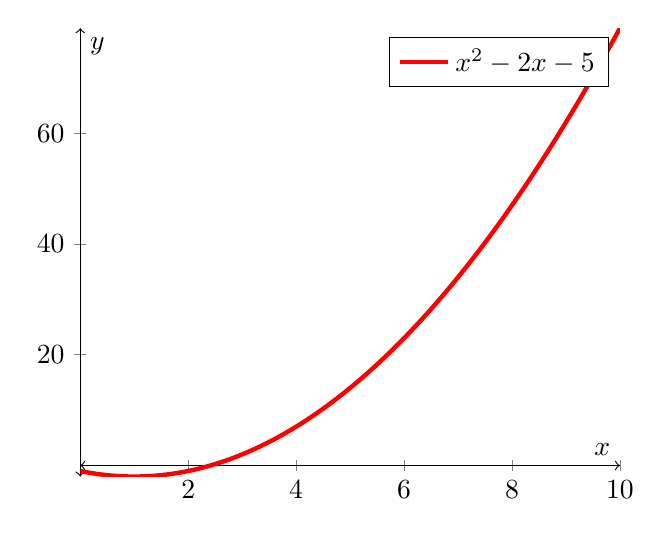
\begin{tikzpicture}
  \begin{axis}
    [
        axis x line=middle,
        axis y line=middle,
        axis line style=<->,
        xlabel = $x$,
        ylabel = $y$,
        every axis plot/.append style={ultra thick},
    ]

    \addplot
    [
        domain=0:10, 
        samples=100, 
        color=red,
    ] {x^2 - 2*x - 1};
    \addlegendentry{$x^2 - 2x - 5$}
  \end{axis}
\end{tikzpicture}

\section{Bar}

\Blindtext%

\subsection{Code Snippets}

\Blindtext%
\blindtext%

\begin{strip}
  \centering\noindent
  \begin{minted}[gobble=4]{haskell}
    -- | Convert slash notation to mask
    fromSlash :: Int -> Word32
    fromSlash n = (.&.) 0xffffffff (complement ((rotateR 2 (32 - n + 1)) - 1))
  \end{minted}
  \captionof{Code Snippet}{: Foobar}
\end{strip}

\Blindtext%
\Blindtext%

\subsection{Algorithms}

\Blindtext%
\blindtext%

\begin{algorithm*}
  \caption{Euclid’s algorithm}\label{euclid}
  \begin{algorithmic}[1]
    \Procedure{Euclid}{$a,b$}\Comment{The g.c.d. of a and b}
      \State $r\gets a\bmod b$
      \While{$r\not=0$}\Comment{We have the answer if r is 0}
        \State $a\gets b$
        \State $b\gets r$
        \State $r\gets a\bmod b$
      \EndWhile\label{euclidendwhile}
      \State \textbf{return} $b$\Comment{The gcd is b}
    \EndProcedure
  \end{algorithmic}
\end{algorithm*}

\section{Baz}

\Blindtext%
\Blindtext%

\end{document}
